%
% exemplo genérico de uso da classe iiufrgs.cls
% $Id: iiufrgs.tex,v 1.1.1.1 2005/01/18 23:54:42 avila Exp $
%
% This is an example file and is hereby explicitly put in the
% public domain.
%
\documentclass[cic,tc]{iiufrgs}
% um tipo específico de monografia pode ser informado como parâmetro opcional:
%\documentclass[tese]{iiufrgs}
% monografias em inglês devem receber o parâmetro `english':
%\documentclass[diss,english]{iiufrgs}
% a opção `openright' pode ser usada para forçar inícios de capítulos
% em páginas ímpares
% \documentclass[openright]{iiufrgs}
% para gerar uma versão somente-frente, basta utilizar a opção `oneside':
% \documentclass[oneside]{iiufrgs}
\usepackage[utf8]{inputenc}   % pacote para acentuação
\usepackage{times}              % pacote para usar fonte Adobe Times
\usepackage[alf,abnt-emphasize=bf]{abntex2cite}	% pacote para usar citações abnt
\usepackage{graphicx}          % para inserir imagens
%\usepackage{mathptmx}          % p/ usar fonte Adobe Times nas fórmulas

\graphicspath{ {images/} }

\title{Uma análise dos dados de queimada do INPE no Brasil (preliminar)}
\translatedtitle{Using \LaTeX\ to Prepare Documents at II/UFRGS}

\author{Braz}{José Henrique da Silva}
\advisor[Prof.~Dr.]{Schnorr}{Lucas M.}

% a data deve ser a da defesa; se nao especificada, são gerados
% mes e ano correntes
%\date{maio}{2001}

% o nome do curso pode ser redefinido (ex. para TCs)
\course{Curso de Graduação em Ciência da Computação}

% o local de realização do trabalho pode ser especificado (ex. para TCs)
% com o comando \location:
\location{Porto Alegre}{RS}

% palavras-chave
% iniciar todas com letras maiúsculas
%
\keyword{Formatação eletrônica de documentos}
\keyword{\LaTeX}
\keyword{ABNT}
\keyword{UFRGS}

%
% palavras-chave na lingua estrangeira
% iniciar todas com letras maiúsculas
%
\translatedkeyword{Electronic document preparation}
\translatedkeyword{\LaTeX}
\translatedkeyword{ABNT}
\translatedkeyword{UFRGS}

%
% inicio do documento
%
\begin{document}

% folha de rosto
% às vezes é necessário redefinir algum comando logo antes de produzir
% a folha de rosto:
% \renewcommand{\coordname}{Coordenadora do Curso}
\maketitle

% dedicatoria
\clearpage
\begin{flushright}
\mbox{}\vfill
{\sffamily\itshape
``If I have seen farther than others,\\
it is because I stood on the shoulders of giants.''\\}
--- \textsc{Sir~Isaac Newton}
\end{flushright}

% agradecimentos
\chapter*{Agradecimentos}
Agradeço ao \LaTeX\ por não ter vírus de macro\ldots

% sumario
\tableofcontents

% lista de abreviaturas e siglas
% o parametro deve ser a abreviatura mais longa
% A NBR 14724:2011 estipula que a ordem das abreviações
% na lista deve ser alfabética (como no exemplo abaixo).
\begin{listofabbrv}{SPMD}
        \item[INPE] Instituto Nacional de Pesquisas Espaciais
        \item[IBGE] Instituto Brasileiro de Geografia e Estatística
        \item[CSV] Comma Separated Values (valores separados por vírgulas).
\end{listofabbrv}

% idem para a lista de símbolos
%\begin{listofsymbols}{$\alpha\beta\pi\omega$}
%       \item[$\sum{\frac{a}{b}}$] Somatório do produtório
%       \item[$\alpha\beta\pi\omega$] Fator de inconstância do resultado
%\end{listofsymbols}

% lista de figuras
\listoffigures

% lista de tabelas
\listoftables

% resumo na língua do documento
\begin{abstract}
Este documento é um exemplo de como formatar documentos para o
Instituto de Informática da UFRGS usando as classes \LaTeX\
disponibilizadas pelo UTUG\@. Ao mesmo tempo, pode servir de consulta
para comandos mais genéricos. \emph{O texto do resumo não deve
conter mais do que 500 palavras.}
\end{abstract}

% resumo na outra língua
\begin{translatedabstract}
This document is an example on how to prepare documents at II/UFRGS
using the \LaTeX\ classes provided by the UTUG\@. At the same time, it
may serve as a guide for general-purpose commands. \emph{The text in
the abstract should not contain more than 500~words.}
\end{translatedabstract}

% aqui comeca o texto propriamente dito

\chapter{Introdução}
P1. Introducao aos dados \par
P2. 


\chapter{Visão geral dos dados}

Neste capítulo constam algumas informações importantes sobre os 
dados disponibilizados pelo INPE, que serão cruciais para compreensão 
dos próximos capítulos. 

\section{O programa DBQueimada}

O DBQueimadas, Banco de Dados de Queimadas (www.inpe.br/queimadas/bdqueimadas),
é um sistema desenvolvido pelo INPE e acessível de forma aberta por meio da web. 
Conta com mais de 300 milhões de pontos coletados desde o ano de 1998, 
proviniente de 32 satélites. Dentro do site é possível gerar mapas,
tabelas, gráficos e exportar os dados aplicando diferentes filtros. Todo o 
programa foi desenvolvido com ferramentas abertas, muitas delas 
criadas pelo próprio time de tecnologia da informação do INPE 
\citep{setzer2019banco}. [P1. Falamos sobre o programa] \par

P2. Ressaltamos a importancia dos dados abertos para a sociedade \par


\section{Garimpando os dados}

Uma parte importante do processo foi coletar os dados do DBQueimadas. 
Para exportar os dados, é necessário preencher os campos de data inicial,
data final e um endereço de e-mail, o intervalo de tempo não 
pode exceder 366 dias. Também é possível aplicar filtros ainda mais 
detalhados como: continente, país, estado, município, satélite, bioma e 
unidades de conservação/terras indígenas. Após clicar em "Exportar", 
uma mensagem é enviada para o e-mail informado com o link de download 
dos dados requisitados. O arquivo disponibilizado é um CSV compactado 
em um zip.\par

Apesar de ser um site fácil de usar e intuitivo, seria praticamente 
inviável baixar todos os dados do Brasil de forma manual. Nesse sentido, 
foi necessário entender quais eventos são disparados quando é feito o 
pedido dos dados a partir da aba "Exportar dados" a fim de automatizar 
o processo de download dos documentos. \par

para isso foi usado um script em Python dividido em 3 etapas:
1. Gerar um arquivo em que cada linha representa uma data de início e de fim
para ser usada no filtro de data para o pedido.



P1. Falar sobre os scripts de coleta dos dados \par
P2. Processo de baixar os dados para o computador \par

\section{Estrutura dos dados}


P1. Aqui da pra usar as perguntas frequentes 
do INPE \citep{PerguntasFrequentesINPE} \par
P2. Falar sobre a flag risco de fogo e uma ideia de como é calculada \par

O dados estão estruturados da seguinte forma: \par

\begin{table}[h!]
\centering
\begin{tabular}{ | l l l | }
\hline
 Coluna & Tipo & Descrição \\
\hline
 Id & string & aaa\\
 Latitude & double & \\ 
 Longitude & double & \\  
 DataHora & string & \\   
 Municipio & string & \\
 Estado & string & \\
 Pais & string & \\  
 Bioma & string & \\
 Precipitação & string & \\
 DiasSCh & integer & \\
 RiscoFog & double & \\
 FRP & double & \\
 \hline
\end{tabular}
\caption{Significado de cada coluna dos dados de queimada do INPE}
\label{table:inpeColumns}
\end{table}

\subsection{Carregando os dados para o Python} 

P1. Aqui pode deve ter código em python \par
P2. Dar uma noção da quantidade de dados \par

\section{Os Satélites}

P1. Satelite de referencia é o AQUA\_M-T \citep{PerguntasFrequentesINPE} \par
P2. Falar sobre os outros principais \par
P3. visão geral dos sensores e porque geram dados diferentes \par
P4. Mostrar gráficos que indicam as horas das coletas

\begin{figure}
    \caption{Relação do montante dos dados por satélite}
    \begin{center}
        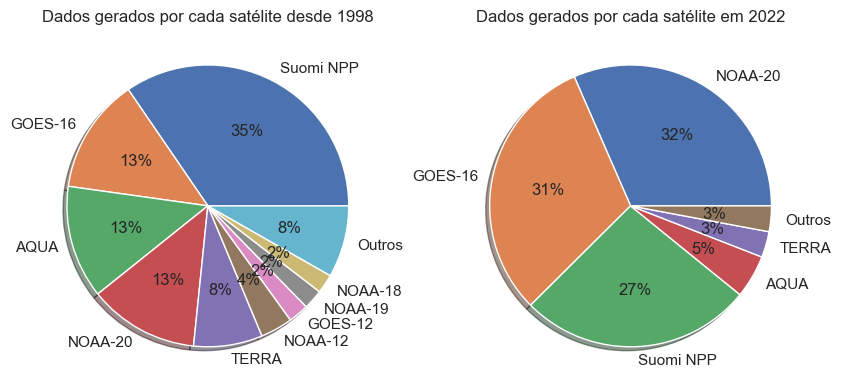
\includegraphics[width=25em]{porcentagem_satelites}
    \end{center}
    \legend{Fonte: Os Autores}
    \label{fig:porcentagem_satelites}
\end{figure}

\section{O que os dados gritam}

P1. Fazer análise preliminar dos dados gerando alguns gráficos \par
P2. Gráficos geral do brasil com os focos de queimadas totais \cite{geographicDataSciencePython} \par


\chapter{Aprofundando a análise dos dados}

aqui a gente mostra que é válido usar esses dados para analises aprofundadas

\section{Densidade e Centrografia}

P1. Verificar densidade e centrografia: tendências, dispersão, extensão \par

\section{Validade dos dados}

Precisamos verificar que os dados seguem algum padrão para ser possível
user eles para tomadas de decisões (garantir que não é aleatório) 
\cite[Point Pattern Analysis]{geographicDataSciencePython} \par

\section{Padronizando os dados por satélite}

P1. Verificar relação entre dados dos diferentes satélites (se possível) e talvez restringir a análise apenas ao satélite de referencia se for identificado que são basicamente equivalentes \par

\chapter{Correlações}

P1. Levantar variáveis que podem influenciar nas queimadas \par
P2. Variáveis humanas: influencia da agricultura, pecuária, 
urbanização, áreas de preservação, reservas indígenas \par
P3. Variáveis naturais: Clima, ondas solares, períodos de chuvas/secas \par



\bibliographystyle{abntex2-alf}
\bibliography{biblio}

\end{document}
